\section{Introduction} \label{sec:intro}

There is a perceived  risk that LSST  images may be snooped during transmission from the telescope. This concerns the images used for alert processing which are transmitted within a minute and provide a valuable resource for identifying moving objects including satellites. Though our processing will ignore satellites other parties may be interested in this information.

In an email during September 2019 Steve Kahn indicated that all data should be encrypted. This would include transfers to Europe.


\subsection{Baseline }
The Rubin Observatory construction project has been built with academic level security in mind.
The
 Information classification policy \citeds{LPM-122} classifies data as  “User Protected”.
The DM Information Security plan \citeds{LDM-324} states the “majority of network traffic will not require confidentiality“

Since our astronomy data is research data with no intrinsic value no great efforts have been made to secure the
data nor the network it is traveling on.
The network has been designed, and now largely implemented, for high throughput not for high security.

The baseline is for encryption of controls but not data i.e. authentication is encrypted, data transmission is not.

{\bf It would be extremely useful if we agreed on the security rating of LSST data (or subsets of it)  as per NIST  \citep{nist800-60}}.
Naively one would assume the security objective would be \emph{Availability}, the potential impact would be \emph{low} for confidentiality, availability and integrity. Hence  the Security Category (SC) would be \{low,low,low\} in NIST terms.

\section{Which data is sensitive ?} \label{sec:which}

In communications thus far and in the security summit held on 6$^{th}$ April 2020 all data has been considered.

Since then the idea of an Alert Vetting System (AVS) to be implemented by LLNL has been raised.
A certain set of of potential alerts  would be sent to  and evaluated by AVS.
These would include  all streaks unattributable to known asteroids that
\begin{enumerate}
\item correspond to objects moving faster than vMax=30 deg/day, or
\item  whose velocity cannot be determined (e.g., due to overlaps with chip boundary).
\end{enumerate}
Streaks not forwarded to the AVS would be published as per current baseline.
Forwarded streaks would be eliminated from Rubin’s public prompt alert stream.
They would also be held back from the publicly queryable Prompt Processing Database (PPDB) for either as long as the focal plane data hasn’t been released  or until the AVS explicitly permits their publication.

\rec{OPS}{AVS}{The operations team with LLNL shall design and implement an Alert Vetting System(AVS).} { Data Production  shall send a subset of potential alerts to LLNL for processing via the AVS, which will run at that separate facility. LLNL will check those alerts against their catalog of assets and flag alerts that should not be issued before the embargo time expires. Rubin should send the alert packets as generated; a list of all the alert packet IDs with a Boolean hold flag should be returned to DP. At a later stage (end of night) a list of images to be embargoed for a longer period should also be returned.}

\subsection{Delaying focal plane data}
We believe the vast majority of the 20TB of nightly images are not of a sensitive nature however we understand the wish is to hold all images in an encrypted store for at least 1 to 3 days.
We understand AVS may embargo some images for up to 30 days based on the streaks found in them.

\rec{DM}{dstore}{ DM shall  implement a  delayed data store. }{
The delayed data store will need to hold images on encrypted disks for an embargo period of between 1 and 30 days.
}




\section{Network security}\label{sec:net}

\begin{figure}
\begin{center}
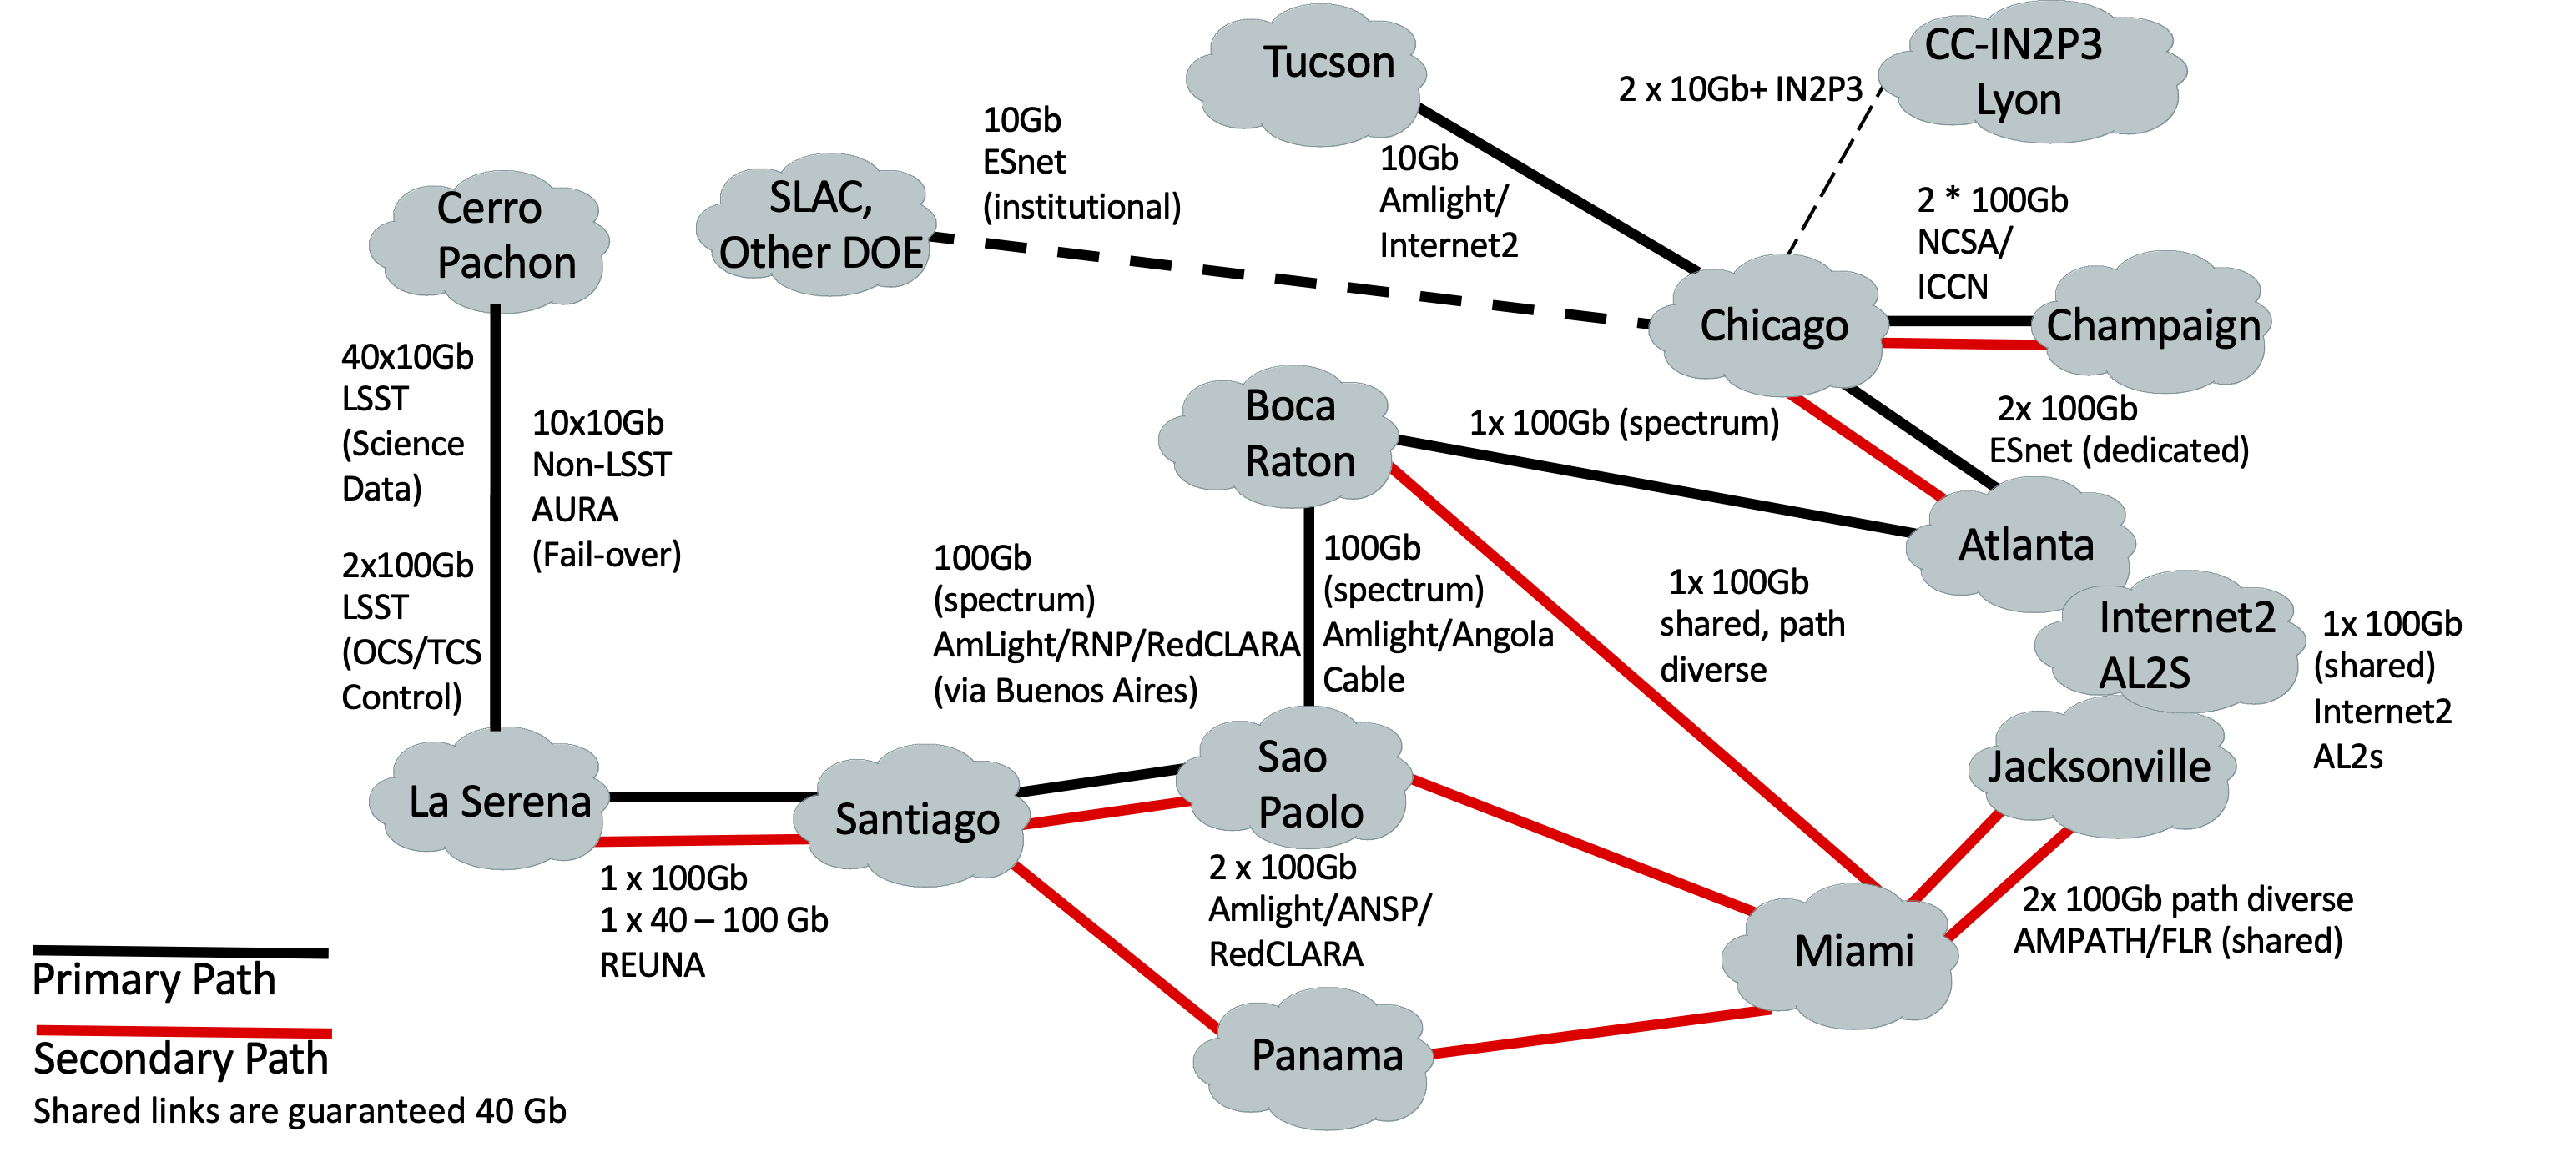
\includegraphics[width=1.0\textwidth]{NetworksFY22}
\caption{Rubin Observatory Network topology for FY22, the primary route is on dedicated lines, the back route is on shared equipment. Securing this beyond the level of the provider will be close to impossible.  \label{fig:net}}
\end{center}
% original https://docs.google.com/presentation/d/1wIN6Dj_rPn8TASBUkAm6_-Yh255Gz9VbwFi61t4LCFs/edit#slide=id.g55f7c0247e_0_2
\end{figure}

On the mountain and in the base facility LSST networks and computers are in rooms requiring ID card access and the compounds
have 24/7 security staff.
We could increase security but it would be costly and probably not very popular with staff i.e it would require raising the security level of the entire facility to something like FSL\footnote{\url{https://emilms.fema.gov/IS1172/groups/85.html}} 2 .

The transfers from Summit to Base and Base to NCSA go over private networks that are not part of the public Internet. We have our own dedicated fibers running from the mountain to the base \citedsp{LSE-78},
intercepting transfers would require physical access to the fibers - tapping those would probably disrupt our network at least temporarily.
For an added security we could also monitor fiber attenuation.
The network is also actively monitored with Bro\footnote{\url{https://www.corelight.com/about-bro/how-bro-works/}} system. Hence we would at least known something was up.
Though technically feasible by perhaps bribing or coercing staff somewhere this seems unlikely - a physical tap should also be noticed during fiber inspections.  The image as transferred over this line is also in an obscure format (though could be put together with some effort).


International transfers to IN2P3 are still being worked out at this time. This may be done on shared commercial carrier. One assumes
this is relatively secure though not perhaps as secure as our dedicated lines. ESNet could be used for this transfer as well if it did not originate at NCSA. There seems no particular reason to do this transfer from NCSA as opposed to directly from Chile or landing it
temporarily at some ESNet endpoint. One may consider the open storage network \citep{osn} for this also though its not currently the baseline.


\section{Transmission security} \label{sec:trans}

It has been indicated, through DOE, that holding data for some time before releasing to the collaboration is an acceptable approach to securing the images - this can be ensured by limiting the LSST personnel who have access to the files during the night.
We would transmit images for alert processing in near realtime to NCSA. We have suggested a six hour delay - there has been no indication of how long the delay needs to be - is one hour sufficient to prevent detection of satellite maneuvers ?

Currently alert images from the base are to be transmitted using BBCP\footnote{BBCP is an alternative to Gridftp when transferring large amounts of data}. The control channel is encrypted but the data channel is open - this is considered secure in the scientific world \citep{bbcp}. Hence theoretically packets snooped on their way to Illinois could be extracted and processed.


Our preference would be to do this in software using TLS based protocols such as HTTPS or FTPS to replace BBCP. This may cause some performance hit.
We could encrypt the data  channel. This would cost us in  compute but could be similar to compression and not push up the number of cores needed for transfer. We would also have some software modification and setup there are projects like WireGuard\footnote{\url{https://www.wireguard.com/}} intending to do this at the kernel level but they are not suitable for Rubin use yet.
There are also  examples of hardware solutions for this which would probably be affordable, INRIA in \cite{10.1007/978-3-642-45073-0_1} have build a FPGA based AES\cite{aes} implementation  which gives 100Gbit/s network rates with $\mu s$ additional latency. Table 3 of \cite{10.1007/978-3-642-45073-0_1} lists the hardware which looks modest enough - we work with INRIA already. There is no price given in the document, but considering the cost of components and a contract to put it together one \emph{might} consider it to be  under \$1M, but we would need to get a quote. This is probably more complex than we might want to get into.

We could encrypt the images themselves before transmission or even on the FPGA of the camera data acquisition (DAQ) system.  The DAQ is complex construction prone to delays so we would rather not jeopardize the project by introducing changes there. Encrypting the files outside would mean more CPU and I/O - it would add a delay in the alerts processing - it may take as much as 20\% of the alerts time budget (1 minute).  This would not be very welcome in the science community. This would require some effort on our side to add encryption to the processing chain but this should be order some hundreds \$K depending on how \emph{secure} it is required to be.



\subsection{Keeping it in Chile}\label{sec:chile}
The original baseline was to do alert processing in Chile in the base facility. Some years ago support for computing in Chile was sub optimal but has improved significantly - there is space in the base facility to hold machines for this.
This would make the base data center the prime target of any data  attack so we may need to review security there.
However if we agree the base/summit are secure we could avoid on the wire snooping by doing alert processing in the base facility. We would also then have to hold images there for the appointed embargo time  before releasing them to the community. We would need to do some work on the cost impacts of this but they should not be insurmountable.


\section{High level summary}\label{sec:sum}
Though the reason behind the call for security and the level required remain totally unclear
NSF and DOE asked for a brief summary of possibilities.
One should also consider which data we are talking about see \secref{sec:which}.
Items here are not costed but an indication is given in terms of low (possibly within cost), moderate (some \$100Ks), high (>\$1M)
Any change should be properly costed.


\begin{longtable}{p{0.75\textwidth} p{0.25\textwidth}}\hline
\textbf{Security idea} & \textbf{Rough cost level}  \\\hline
 {\bf Delay some or all images.} Depending on how secure this needs to be and where it is done the cost scales.  & Low to Moderate.\\
 {\bf Do alerts in Chile.} If we want to control image access for a longer period we could consider alert production in Chile. The hardware budget would remain the same but we may require extra support in Chile.  & Low to Moderate.\\
{\bf Encrypt all images.} This would have to be done on the summit or in la Serena before hitting the long haul network. Possibly no new hardware needed but a change in software.  & Can be Low \\
{\bf Transmission Layer Encryption.} Network encryption would probably require new hardware. & Moderate \\
{\bf Physically securing the network.} This will be next to impossible and would probably require new network agreements. This however would be the only way to ensure no packet snooping. & Very high \\
{\bf Avoid certain time coordinates.} This would require changing the scheduler to provide more constraints on pointing. &  Moderate  \\\hline
\end{longtable}

